% MATH 573 HW 3
% LUKE WUKMER

\documentclass[10pt]{article}

% note: some of these are extremely useful and i don't remember why :o
%\usepackage{savetrees} % disable custom geometry stuff if you do this
\usepackage{titling}    % contol over title & stuff
\usepackage{amsmath, amsthm, amssymb, amsfonts}
\usepackage{amsxtra, amscd, geometry, graphicx}
\usepackage{endnotes}
\usepackage{cancel}
\usepackage{wrapfig}    %inline figs
\usepackage{bm} %allows fancy stuff like bold greek in math mode
\usepackage{alltt}
\usepackage{enumerate} %more/easier control over lists, also see enumitem
%\usepackage[all,cmtip]{xypic}
\usepackage{mathrsfs}
\usepackage{listings}
\usepackage{caption}
%\usepackage{subfigure}
%\usepackage{subcaption}
%\usepackage[pdftex]{hyperref}
%\usepackage[dvips,bookmarks,bookmarksopen,backref,colorlinks,linkcolor={blue},citecolor={blue},urlcolor={blue}](hyperref}


\usepackage{color}

\definecolor{mygreen}{rgb}{0,0.6,0}
\definecolor{mygray}{rgb}{0.5,0.5,0.5}
\definecolor{mymauve}{rgb}{0.58,0,0.82}

\lstset{ %
  backgroundcolor=\color{white},   % choose the background color; you must add \usepackage{color} or \usepackage{xcolor}
  basicstyle=\footnotesize,        % the size of the fonts that are used for the code
  breakatwhitespace=false,         % sets if automatic breaks should only happen at whitespace
  breaklines=true,                 % sets automatic line breaking
  captionpos=b,                    % sets the caption-position to bottom
  commentstyle=\color{mygreen},    % comment style
  deletekeywords={...},            % if you want to delete keywords from the given language
  escapeinside={\%*}{*)},          % if you want to add LaTeX within your code
  extendedchars=true,              % lets you use non-ASCII characters; for 8-bits encodings only, does not work with UTF-8
  frame=single,	                   % adds a frame around the code
  keepspaces=true,                 % keeps spaces in text, useful for keeping indentation of code (possibly needs columns=flexible)
  keywordstyle=\color{blue},       % keyword style
  language=Python,                 % the language of the code
  otherkeywords={*,...},           % if you want to add more keywords to the set
  numbers=left,                    % where to put the line-numbers; possible values are (none, left, right)
  numbersep=5pt,                   % how far the line-numbers are from the code
  numberstyle=\tiny\color{mygray}, % the style that is used for the line-numbers
  rulecolor=\color{black},         % if not set, the frame-color may be changed on line-breaks within not-black text (e.g. comments (green here))
  showspaces=false,                % show spaces everywhere adding particular underscores; it overrides 'showstringspaces'
  showstringspaces=false,          % underline spaces within strings only
  showtabs=false,                  % show tabs within strings adding particular underscores
  stepnumber=2,                    % the step between two line-numbers. If it's 1, each line will be numbered
  stringstyle=\color{mymauve},     % string literal style
  tabsize=2,	                   % sets default tabsize to 2 spaces
  title=\lstname                   % show the filename of files included with \lstinputlisting; also try caption instead of title
}
% change up the fonts (pick one only)
%\usepackage{times}%
\usepackage{helvet}%
%\usepackage{palatino}%
%\usepackage{bookman}%


% These are italic.
\theoremstyle{plain}
\newtheorem{thm}{Theorem}
\newtheorem*{thm*}{Theorem}
\newtheorem{prop}{Proposition}
\newtheorem*{prop*}{Proposition}
\newtheorem{conj}{Conjecture}
\newtheorem*{conj*}{Conjecture}
\newtheorem{lem}{Lemma}
  \makeatletter
  \@addtoreset{lem}{thm}
  \makeatother 
\newtheorem*{lem*}{Lemma}
\newtheorem{cor}{Corollary}
  \makeatletter
  \@addtoreset{cor}{thm}
  \makeatother 
\newtheorem*{cor*}{Corollary}

%\newtheorem{lem}[thm]{Lemma}
%\newtheorem{remark}[thm]{Remark}
%\newtheorem{cor}[thm]{Corollary}
%\newtheorem{prop}[thm]{Proposition}
%\newtheorem{conj}[thm]{Conjecture}

% These are normal (i.e. not italic).
\theoremstyle{definition}
\newtheorem*{ack*}{Acknowledgements}
\newtheorem*{app*}{Application}
\newtheorem*{apps*}{Applications}
\newtheorem{defn}{Definition}
\newtheorem*{defn*}{Definition}
\newtheorem{eg}{Example}
  \makeatletter
  \@addtoreset{eg}{thm}
  \makeatother 
\newtheorem*{eg*}{Example}
\newtheorem*{egs*}{Examples}
\newtheorem{ex}{Exercise}
\newtheorem*{ex*}{Exercise}
\newtheorem*{quest*}{Question}
\newtheorem{rem}{Remark}
\newtheorem*{rem*}{Remark}
\newtheorem{rems}{Remarks}
\newtheorem*{rems*}{Remarks}
\newtheorem{prob}{Problem}
\newtheorem*{prob*}{Problem}
\newtheorem*{soln*}{Solution}
\newtheorem{soln}{Solution}


% New Commands: Common Math Symbols
\providecommand{\R}{\mathbb{R}}%
\providecommand{\N}{\mathbb{N}}%
\providecommand{\Z}{{\mathbb{Z}}}%
\providecommand{\sph}{\mathbb{S}}%
\providecommand{\Q}{\mathbb{Q}}%
\providecommand{\C}{{\mathbb{C}}}%
\providecommand{\F}{\mathbb{F}}%
\providecommand{\quat}{\mathbb{H}}%

% haha, i originally forked this template from one provided by my abstract
% algebra TA (back in 2012 or something). probably don't need most of these,
% huh. 

% New Commands: Operators
\providecommand{\Gal}{\operatorname{Gal}}%
\providecommand{\GL}{\operatorname{GL}}%
\providecommand{\card}{\operatorname{card}}%
\providecommand{\coker}{\operatorname{coker}}%
\providecommand{\id}{\operatorname{id}}%
\providecommand{\im}{\operatorname{im}}%
\providecommand{\diam}{{\rm diam}}%
\providecommand{\aut}{\operatorname{Aut}}%
\providecommand{\inn}{\operatorname{Inn}}%
\providecommand{\out}{{\rm Out}}%
\providecommand{\End}{{\rm End}}%
\providecommand{\rad}{{\rm Rad}}%
\providecommand{\rk}{{\rm rank}}%
\providecommand{\ord}{{\rm ord}}%
\providecommand{\tor}{{\rm Tor}}%
\providecommand{\comp}{{\text{ $\scriptstyle \circ$ }}}%
\providecommand{\cl}[1]{\overline{#1}}%
\providecommand{\tr}{{\sf trace}}%

\renewcommand{\tilde}[1]{\widetilde{#1}}%
\numberwithin{equation}{section}

% i like the squiggly ones more. add as needed

\renewcommand{\Psi}{\varPsi}

\newcommand*\rfrac[2]{{}^{#1}\!/_{#2}}

% a very fancy dot product \ip{f}{g}
\newcommand\ip[2]{ \left\langle {#1} , {#2} \right\rangle }

% "s.t." for math mode
\providecommand{\st}{\text{ s.t. }}

% \norm{f} and such, super useful
\newcommand{\norm}[1]{\left\lVert#1\right\rVert}

% determinant
%\newcommand{\det}[1]{\textsf{det}\left(#1\right)}

% jacobian
\providecommand{\J}{\textsf{J}}

% this makes the spacing between lines of font a little bigger
%\newcommand{\spacing}[1]{\renewcommand{\baselinestretch}{#1}\large\normalsize}
%\spacing{1.2}

\newcommand*\mcol[1]{\overset{\big\uparrow}{\underset{\big\downarrow}{#1}}}

% Makes the margin size a little smaller, i gots stuff to say
\geometry{letterpaper,margin=.8in}

% titling stuff (from package titling)
\posttitle{\par\end{center}}
\setlength{\droptitle}{-.5in}
% END PREAMBLE %%%%%%%%%%%%%%%%%%%%%%%%%
%%%%%%%%%%%%%%%%%%%%%%%%%%%%%%%%%%%%%%%%


\begin{document}

\title{Math 573 HW\textsuperscript{\#}3}
\author{Luke Wukmer}
\date{Fall 2015}
\maketitle \thispagestyle{empty} % remove the page number from the first page
\lstset{language=Python}

%%% PROBLEM 1
\begin{prob}
    A least squares polynomial of degree $\leq n$ is some $p_n(x) = \sum_{k=0}^n a_k x^k$
    is one that minimizes the least-squared error
    $E_2(\bm{a}) := \sum_{i=1}^{m}\left[p_n(x_i) - y_i\right]^2$
    for some $m \geq n+1$ data points $(x_i, y_i)$.  
    This optimal solution is found in terms of the coefficients
    $\bm{a} := (a_i) \in \R^{(n+1) \times 1}$ by solving the normal equation
    \[      
            \mathbb{X}^T\mathbb{X}\, \bm{a} = \mathbb{X}^T \bm{y}
    \]
    where \[
            \mathbb{X} := \begin{bmatrix}
                \uparrow & \uparrow & \uparrow &    & \uparrow \\
            1       & x_i & (x_i)^2 & \cdots & (x_i)^n      \\\
            \downarrow & \downarrow & \downarrow &  & \downarrow 
            \end{bmatrix}_{(m \times (n+1))} , \quad
        \bm{y} := \begin{bmatrix}\mcol{y_i}\end{bmatrix}_{(m \times 1)}
\]
We demonstrate this solution method by finding several least squares approximations of the
following data ($m=4$):
    \begin{center}
        \begin{tabular}{c c c c c}
        \hline
        $x_i$ & 1.0 & 1.1 & 1.3 & 1.5 \\
        $y_i$ & 1.84 & 1.96 & 2.21 & 2.45\\
        \hline
    \end{tabular} 
    \end{center}
\begin{enumerate}[\bfseries(a)]
\item $n=2$: We find 
    \[
            \mathbb{X} = \begin{pmatrix}
                1 & 1.0 & (1.0)^2 \\
                1 & (1.1) & (1.1)^2 \\
                1 & (1.3) & (1.3)^2 \\
                1 & (1.5) & (1.5)^2 \\
            \end{pmatrix}
            \quad \Longrightarrow \quad
            \mathbb{X}^T\mathbb{X} = 
            \begin{pmatrix} 
            4.    &   4.9   &   6.15  \\
            4.9   &   6.15  &   7.903 \\
            6.15  &   7.903 &  10.3827\\
        \end{pmatrix}
            \]
    \[
        \mathbb{X}^T \bm{y} = \mathbb{X}^T \begin{bmatrix} 1.84 \\ 1.96 \\ 2.21 \\ 2.45 \end{bmatrix}
        = \begin{pmatrix}8.46 \\  10.544 \\  13.459 \end{pmatrix}
        \]
    Thus we have the system
    \[
            \left(\mathbb{X}^T\mathbb{X}\right)\bm{a} = 
            \begin{pmatrix} 
            4.    &   4.9   &   6.15  \\
            4.9   &   6.15  &   7.903 \\
            6.15  &   7.903 &  10.3827\\
            \end{pmatrix} \begin{bmatrix} a_0 \\ a_1 \\ a_2 \end{bmatrix}
        = \begin{pmatrix}8.46 \\  10.544 \\  13.459 \end{pmatrix}
        = \mathbb{X}^T \bm{y}
    \]

    whose solution (by Gaussian elimination or what-have-you) is
    $\bm{a} = \begin{bmatrix} 0.55253769  & 1.32751256 & -0.04145729\end{bmatrix}^T$,
    corresponding to the polynomial
    \[
            \boxed{y = p_2(x) := 0.55253769 + 1.32751256 \,x - 0.04145729\, x^2}
        \]
        This polynomial is plotted along with the the control points $(x_i, y_i)$
        in \textbf{Figure 1}.
        The associated error is
        $E_2(\bm{a}) = \sum_{i=1}^m \left[\, p_2(x_i) - y_i\, \right]^2 = 1.23115577889\mathsf{e}-5$.
\item $n=3$:
    Similarly, we obtain 
    \[
            \mathbb{X} = \begin{pmatrix}
                1 & 1.0 & (1.0)^2  & (1.0)^3\\
                1 & (1.1) & (1.1)^2 & (1.1)^3\\
                1 & (1.3) & (1.3)^2 & (1.3)^3\\
                1 & (1.5) & (1.5)^2 & (1.5)^3\\
            \end{pmatrix}
            \quad \Longrightarrow \quad
            \mathbb{X}^T\mathbb{X} = 
        \begin{pmatrix}
        4.      &   4.9     &   6.15    &   7.903   \\
        4.9     &   6.15    &   7.903   &  10.3827  \\
        6.15    &   7.903   &  10.3827  &  13.91719 \\
        7.903   &  10.3827  &  13.91719 &  18.988995
        \end{pmatrix}
            \]
    \[
        \mathbb{X}^T \bm{y} = \mathbb{X}^T \begin{bmatrix} 1.84 \\ 1.96 \\ 2.21 \\ 2.45 \end{bmatrix}
        = \begin{pmatrix}8.46 \\  10.544 \\  13.459 \\ 17.57288 \end{pmatrix}
        \]
%\[
%   \begin{bmatrix}
%       4          & \sum (x_i)   & \sum x_i^2 & \sum x_i^3 \\
%       \sum x_i   & \sum (x_i)^2 & \sum x_i^3 & \sum x_i^4 \\
%       \sum x_i^2 & \sum (x_i)^3 & \sum x_i^4 & \sum x_i^5 \\
%       \sum x_i^3 & \sum (x_i)^4 & \sum x_i^5 & \sum x_i^6 \\
%   \end{bmatrix}
%   \begin{bmatrix} a_0 \\ a_1 \\ a_2 \\ a_3 \end{bmatrix}
%   =
%   \begin{bmatrix} \sum y_i \\ \sum y_i x_i \\ \sum y_i x_i^2 \\ \sum y_i x_i^3 \end{bmatrix}
%   \]
        And so we have the system
\[
\begin{pmatrix}
4.      &   4.9     &   6.15    &   7.903   \\
4.9     &   6.15    &   7.903   &  10.3827  \\
6.15    &   7.903   &  10.3827  &  13.91719 \\
7.903   &  10.3827  &  13.91719 &  18.988995
\end{pmatrix}
\begin{bmatrix} a_0 \\ a_1 \\ a_2 \\ a_3 \end{bmatrix}
= \begin{pmatrix} 8.46    \\ 10.544   \\ 13.459   \\ 17.57288 \end{pmatrix}
\]
whose solution is
$\bm{a} = \begin{bmatrix} 1.6575 & -1.38416667 & 2.15 & -0.58333333 \end{bmatrix}^T$. Thus
the least-squares polynomial of degree 3 is
\[
        \boxed{y = p_3(x) := 1.6575  - 1.38416667 x + 2.15 x^2  - 0.58333333 x^3}
\]
        with least squares error
        $E_2(\bm{a}) = \sum_{i=1}^m \left[\, p_2(x_i) - y_i\, \right]^2 =
            8.757064 \mathsf{e}-24$.
            We plot this polynomial with the control points $(x_i, y_i)$
            in \textbf{Figure 2} below.  \item   $y= bx^a$ form:
    Solving the equations $\frac{\partial E_2}{\partial a} = 0 , \frac{\partial E_2}{\partial b} = 0$
    involves a nasty system of nonlinear equations, so we search for the
    linearized form of our target equation. \textbf{Continue the mild derivation.}

    The solution of the system is
    \[\boxed{p(x) = (1.8362676528) x^{0.708717475596}}\]
    with least squares error
    $E_2(\bm{a}) = \sum_{i=1}^m \left[\, p(x_i) - y_i\, \right]^2 =  4.31903088848\mathsf{e}-05$.
    See figure 3.
\item Comparing the least squared errors, it seems the polynomial of degree 3 gives the best fit.
\end{enumerate}

\end{prob}

\hrulefill
%%% PROBLEM 2
\begin{prob}
    A cardinal spline is a sequence of individual curves joined to form a
    larger curve. The spline is specified by an array of points and a tension
    parameter, $c$. A cardinal spline passes smoothly through each point in the
    array; there are no sharp corners and no abrupt changes in the tightness
    of the curve. A cardinal spline (often used to make a polygon) uses an
    alternative formula for calculating the tangents at each interval
    (compared to Hermite curves). In particular, 
    \[
            m_k = \frac{1}{2}(1-c)\left(P_{k+1} - P_{k-1}\right)
        \]
    is used to calculate the tangent at $P_k$, where $c$ is between 0 and 1.
    Find the blending functions of the cardinal splines.
\end{prob}

\begin{soln*}
    We formulate a sequence of cardinal splines for some control points
    $\{P_k\}_{k=1}^{N} \subset \R^3$ and
    a fixed tension parameter $c \in {[0,1)}$. For $ 1 < k < N-1$,
        our goal is to create a spline $\bm{p}_k(t)$ between the points
        $P_k$ and $P_{k+1}$ satisfying the following: 
    \begin{gather*}
    \bm{p}_k: {[0,1]} \rightarrow \R^3 \quad \st \quad
    \bm{p}_k(0) = P_k , \; \bm{p}_k(1) = P_{k+1} , \\
    \bm{p}'(0) = m_k = \frac{1}{2}(1-c)\left(P_{k+1} - P_{k-1}\right) \quad
    \bm{p}'(1) = m_{k+1} = \frac{1}{2}(1-c)\left(P_{k+2} - P_{k}\right) 
    \end{gather*}
    From these contraints we see that each $\bm{p}_k(t)$ is specified by the geometry
    $G_C := \begin{bmatrix} P_{k-1} & P_k & P_{k+1} & P_{k+2} \end{bmatrix}^T$.
    Using the conditions above, we can readily convert between the geometries
    of Hermite/cardinal by the defining the matrix $M_{HC}$, where
    \[
            \underbrace{\begin{bmatrix}
                0 & 1 & 0 & 0 \\
                0 & 0 & 1 & 0 \\
                -\frac{1}{2}(1-c) & 0 & \frac{1}{2}(1-c) & 0 \\
                0 & -\frac{1}{2}(1-c) & 0 & \frac{1}{2}(1-c)
                \end{bmatrix}}_{M_{HC}}
            \underbrace{
            \begin{bmatrix}
                P_{k-1} \\ P_k \\ P_{k+1} \\ P_{k+2}
        \end{bmatrix}}_{G_C}
            =
            \underbrace{
            \begin{bmatrix}
                \bm{p}(0) \\ \bm{p}(1) \\ \bm{p}'(0) \\ \bm{p}'(1)
        \end{bmatrix}}_{G_H}
        \]
    We substitute $G_H = M_{HC} G_C$ directly into the solution for Hermite curves, defining a
    $M_C := M_H M_{HC}$:
    \[
            \bm{p}_k(t) = \bm{t}^T C = \bm{t}^T M_H G_H = \bm{t}^T M_H (M_{HC} G_C )
                        = \bm{t}^T M_C G_C 
                        = (M_C^T \bm{t})^T \cdot G_C
        \]
        Explicitly, this $M_C$ becomes
    \begin{align*}
            M_C := M_H M_{HC}
            &= \begin{bmatrix}
                2 & {-2} & 1 & 1 \\
                {-3} & 3 & {-2} & -1 \\
                0 & 0 & 1 & 0 \\
                1 & 0 & 0 & 0 \end{bmatrix}
            \begin{bmatrix}
                0 & 1 & 0 & 0 \\
                0 & 0 & 1 & 0 \\
                -\frac{1}{2}(1-c) & 0 & \frac{1}{2}(1-c) & 0 \\
                0 & -\frac{1}{2}(1-c) & 0 & \frac{1}{2}(1-c)
            \end{bmatrix} \\
            &= 
            \frac{1}{2} \begin{bmatrix}
                (c-1)   & (c+3)     & -(c+3)    & -(c-1)    \\
                -2(c-1) & -(c+5)    & 2(c+2)    & (c-1)     \\
                (c-1)   & 0         & -(c-1)    & 0         \\
                0       & 2         & 0         & 2
            \end{bmatrix}
    \end{align*}
    
    As with Hermite curves, we can define the blending functions
    $\bm{b}(t) = M_C^T \bm{t}$, with
    \begin{align*}
    \bm{b}(t) = M_C^T \bm{t}
              = 
            \frac{1}{2} \begin{bmatrix}
                (c-1)   & -2(c-1)   & (c-1)     & 0         \\
                (c+3)   & -(c+5)    & 0         & 2         \\
                -(c+3)  & 2(c+2)    & -(c-1)    & 0         \\
                -(c-1)  & (c-1)     & 0         & 2
            \end{bmatrix}
    \begin{bmatrix} t^3 \\ t^2 \\ t \\ 1 \end{bmatrix} \\
          =  \frac{1}{2} \begin{bmatrix}
              (c-1)   t^3 -2(c-1) t^2  + (c-1)  t \\ 
              (c+3)   t^3 -(c+5)  t^2    +     t   + 2         \\
              -(c+3)  t^3 + 2(c+2)  t^2  -(c-1) t  \\ 
              -(c-1)  t^3 + (c-1)   t^2  + 2
            \end{bmatrix}
            \begin{matrix}
                =: b_1(t) \\
                =: b_2(t) \\
                =: b_3(t) \\
                =: b_4(t) 
            \end{matrix}
    \end{align*}

    We plot these general blending functions over the interval $t\in[0,1]$ for several values
    of $c$ in \textbf{Figure 4} below.
\end{soln*}
\hrulefill

%%% PROBLEM 3
\begin{prob} \textit{Least-squares on a larger data set}

    Running the file \texttt{p3.py} (renamed \texttt{luke\_Wukmer\_HW3\_Prob3.py} in the submitted material)
    yields the following output:
\begin{verbatim}
wukm@zoo ~/573/hw3 (git)-[master] % python p3.py
line coefficients: [-0.80283142  0.22334848]
linear error =  6153.81704917
exp. coefficients, a=0.8139010446670706, b=0.6284427563244188
exponential error =  6363.48808059
\end{verbatim}

This program uses the least-squares solving implementation found in 
\texttt{least\_squares.py} to find a linear fit and a fit of the form
$y=bx^a$ for the data in \textbf{Table 2} (refer to HW).
This output indidicates that the least-squares line is given by the form
    \[
            y = p_1(x) := (-0.80283142) + (0.22334848)\,x
    \]

with error $E_2 = 6153.82$. Solving for $y$ here yields the predicted HW scores for
a student receiving a $60\%$ and a $90\%$ on the final, respectively:
$(272.6,60), (406.6,90)$.

Similarly, the $y=bx^a$ form given by
    \[
            y = q(x) := 0.62844 \cdot x^{0.81390}
        \]

with error $E_2 = 6363.5$. Solving for $y$ here yields the predicted HW scores for
a student receiving a $60\%$ and a $90\%$ on the final, respectively:
$(270.8,60), (445.6,90)$.

These equations along with the dataset itself are plotted in \textbf{Figure 5}.
Visually, these two forms do not seem to fit the data well
(which corresponds to the large errors obtained for each form).
This large error seems unavoidable. Indeed, we do not intuitively expect there to be a strong,
predictable pattern between HW and exam scores.

\end{prob}

\hrulefill

%%% PROBLEM 4
\begin{prob} \textit{B-splines on a ``mystery'' data set}

    Refer to \textbf{Figure 6} for a plot sequence of b-splines obtained from
    a ``mystery'' data set (refer to HW).
    Notice that the last three data points are identical to the first three,
    so that $p_{N-1}(1) = p_1(0)$ and the splines connect in a loop
    (where $N$ is the size of the data set).
    Upon examining the resulting graph, it appears these data points have been
    carefully chosen so that their b-splines connect in the whimsical shape of a
    puppy.

    For each sequential group of four data points $P_{i}, P_{i+1}, P_{i+2}, P_{i+3}$,
    we apply the b-spline blending functions $\bm{b}(t)$,
    which are given in the function \texttt{blending\_mesh()} in \texttt{bsplines.py}:
    \lstinputlisting[firstline=9]{../bspline.py}
     
    Since we must graph the polynomial using some mesh of $[0,1]$,
    we find it is actually more convenient to apply these blending functions to the mesh directly.
    The result, when dotted with $[P_{i}, P_{i+1}, P_{i+2}, P_{i+3}]$, returns the interpolation points
    of the graphed polynomial itself.

    These functions are used to produce the graph seen in \textbf{Figure 6}:

    \lstinputlisting[firstline=26, lastline=38]{luke_Wukmer_HW3_Prob4.py}

\end{prob}

%%%%%%%%%%%%%%%%%%%%%%%%%%%%%%%%%%%%%%%%%%%%%%%%%%%%%%%%%%%%%%%%%%%%%%%%%%%%%%

\begin{figure}[p]
    \begin{center}
        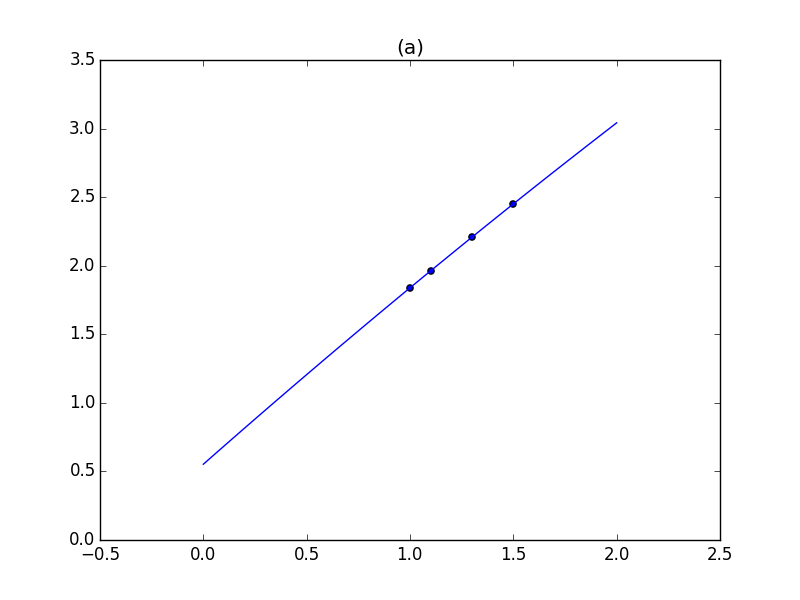
\includegraphics[width=0.8\textwidth]{p1_2}
        \caption{Least squares polynomial degree (2) from \textbf{Problem 1(a)}}
    \end{center}
\end{figure}

\begin{figure}[p]
    \begin{center}
        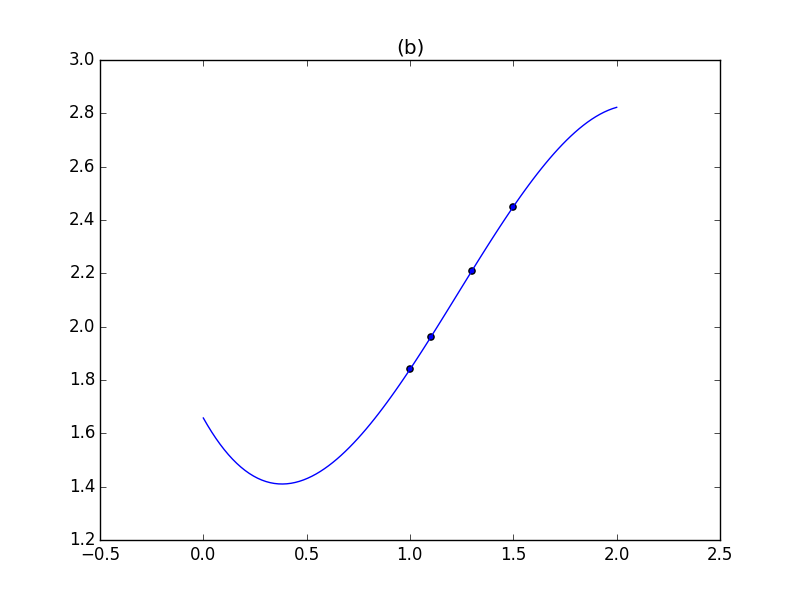
\includegraphics[width=0.8\textwidth]{p1_3}
        \caption{Least squares polynomial degree (3) from \textbf{Problem 1(b)}}
    \end{center}
\end{figure}

\begin{figure}[p]
    \begin{center}
        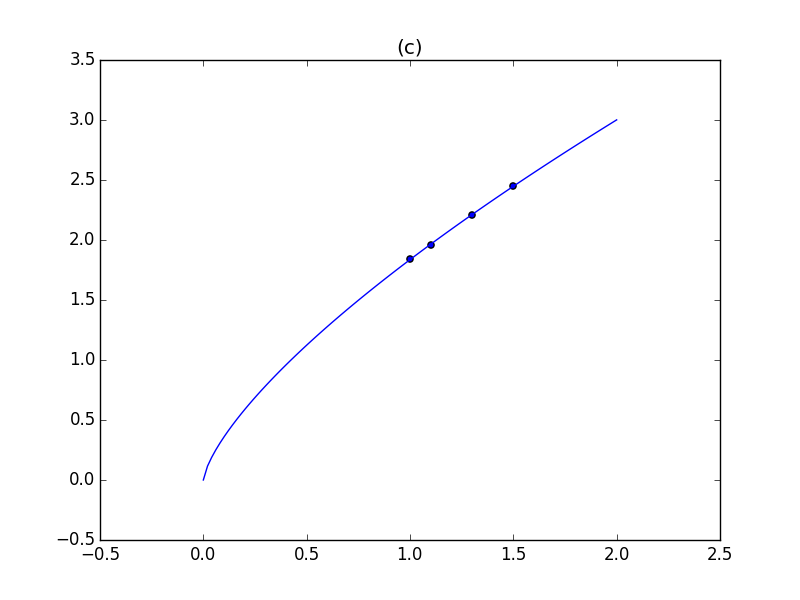
\includegraphics[width=0.8\textwidth]{p1_exp}
        \caption{Least squares (exponential form) from \textbf{Problem 1(c)}}
    \end{center}
\end{figure}

\begin{figure}[p]
    \begin{center}
    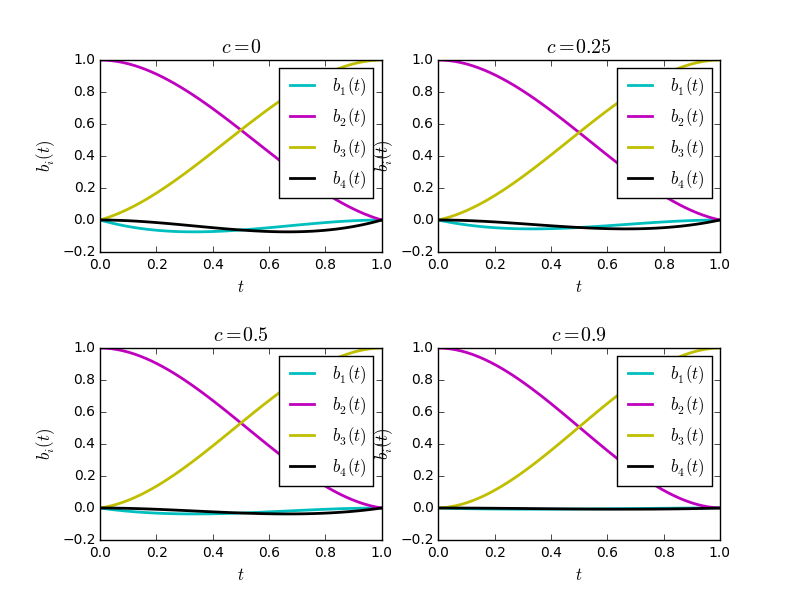
\includegraphics[width=.8\textwidth]{cardinals}
    \caption{Graphing the blending functions of the cardinal spline for several values of $c$.}
    \end{center}
\end{figure}

\begin{figure}[p]
    \begin{center}
        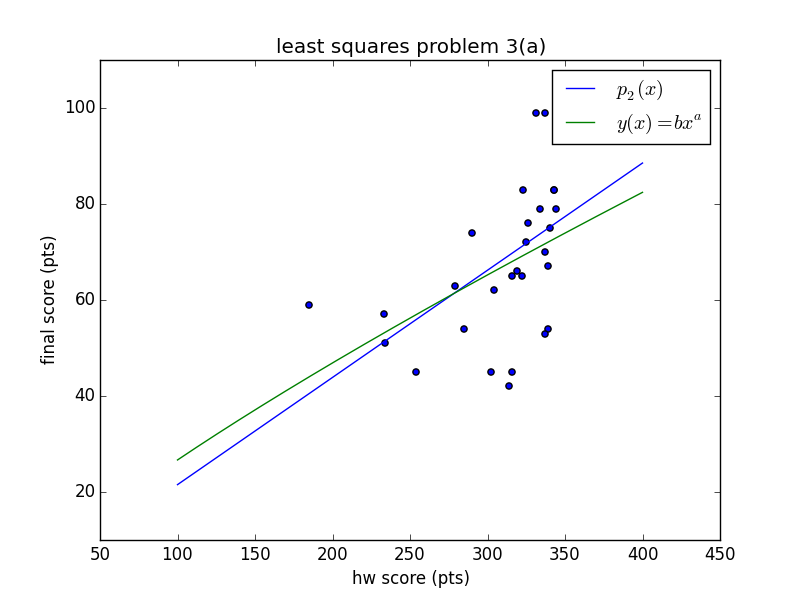
\includegraphics[width=0.8\textwidth]{p3}
        \caption{Graph of the two least-square approximations in \textbf{Problem 3},
        along with the corresponding dataset}
    \end{center}
\end{figure}

\begin{figure}[p]
    \begin{center}
    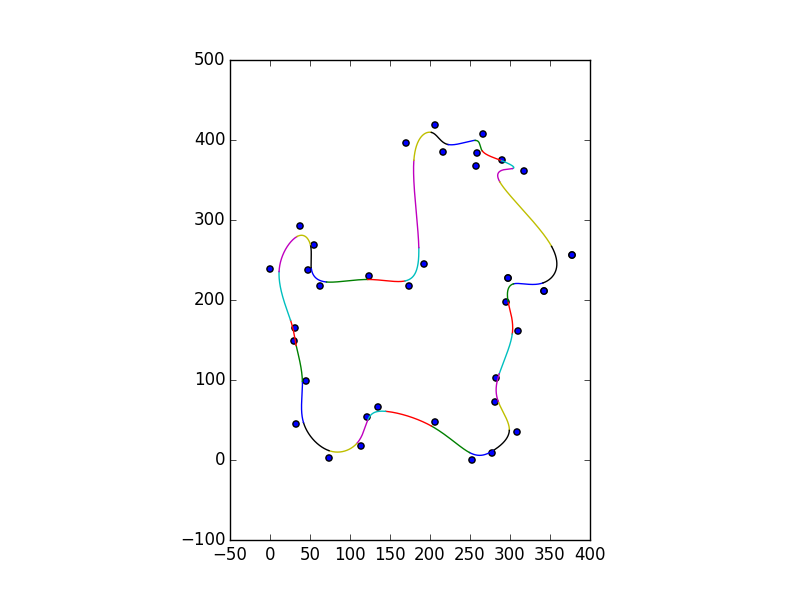
\includegraphics[width=0.8\textwidth]{doggy_splines}
    \caption{B-spline fitting of the doggy-data (see \textbf{Problem 4})}
\end{center}
\end{figure}
%%%%%%%%%%%%%%%%%%%%%%%%%%%%%%%%%%%%%%%%%%%%%%%%%%%%%%%%%%%%%%%%%%%%%%%%%%%%%%
\end{document}
